%  LaTeX support: latex@mdpi.com 
%  In case you need support, please attach all files that are necessary for compiling as well as the log file, and specify the details of your LaTeX setup (which operating system and LaTeX version / tools you are using).

% You need to save the "mdpi.cls" and "mdpi.bst" files into the same folder as this template file.

%=================================================================
\documentclass[entropy,article,submit,moreauthors,pdftex,10pt,a4paper]{mdpi} 

%
%--------------------
% Class Options:
%--------------------
% journal
%----------
% Choose between the following MDPI journals:
% actuators, admsci, aerospace, agriculture, agronomy, algorithms, animals, antibiotics, antibodies, antioxidants, applsci, arts, atmosphere, atoms, axioms, batteries, behavsci, beverages, bioengineering, biology, biomedicines, biomimetics, biomolecules, biosensors, brainsci, buildings, carbon, cancers, catalysts, cells, challenges, chemosensors, children, chromatography, climate, coatings, computation, computers, condensedmatter, cosmetics, cryptography, crystals, data, dentistry, designs, diagnostics, diseases, diversity, econometrics, economies, education, electronics, energies, entropy, environments, epigenomes, fermentation, fibers, fishes, fluids, foods, forests, futureinternet, galaxies, games, gels, genealogy, genes, geosciences, geriatrics, healthcare, horticulturae, humanities, hydrology, informatics, information, infrastructures, inorganics, insects, instruments, ijerph, ijfs, ijms, ijgi, ijtpp, inventions, jcdd, jcm, jdb, jfb, jfmk, jimaging, jof, jintelligence, jlpea, jmse, jpm, jrfm, jsan, land, languages, laws, life, literature, lubricants, machines, magnetochemistry, marinedrugs, materials, mathematics, mca, mti, medsci, medicines, membranes, metabolites, metals, microarrays, micromachines, microorganisms, minerals, molbank, molecules, mps, nanomaterials, ncrna, neonatalscreening, nutrients, particles, pathogens, pharmaceuticals, pharmaceutics, pharmacy, philosophies, photonics, plants, polymers, processes, proteomes, publications, recycling, religions, remotesensing, resources, risks, robotics, safety, sensors, separations, sexes, sinusitis, socsci, societies, soils, sports, standards, sustainability, symmetry, systems, technologies, toxics, toxins, tropicalmed, universe, urbansci, vaccines, vetsci, viruses, water
%---------
% article
%---------
% The default type of manuscript is article, but can be replaced by: 
% addendum, article, book, bookreview, briefreport, casereport, changes, comment, commentary, communication, conceptpaper, correction, conferenceproceedings, conferencereport, expressionofconcern, meetingreport, creative, datadescriptor, discussion, editorial, essay, erratum, hypothesis, interestingimage, letter, newbookreceived, opinion, obituary, projectreport, reply, retraction, review, preprints, shortnote, supfile, technicalnote
% supfile = supplementary materials
%----------
% submit
%----------
% The class option "submit" will be changed to "accept" by the Editorial Office when the paper is accepted. This will only make changes to the frontpage (e.g. the logo of the journal will get visible), the headings, and the copyright information. Also, line numbering will be removed. Journal info and pagination for accepted papers will also be assigned by the Editorial Office.
%------------------
% moreauthors
%------------------
% If there is only one author the class option oneauthor should be used. Otherwise use the class option moreauthors.
%---------
% pdftex
%---------
% The option pdftex is for use with pdfLaTeX. If eps figure are used, remove the option pdftex and use LaTeX and dvi2pdf.

%=================================================================
\firstpage{1} 
\makeatletter 
\setcounter{page}{\@firstpage} 
\makeatother 
\articlenumber{x}
\doinum{10.3390/------}
\pubvolume{xx}
\pubyear{2016}
\copyrightyear{2016}
\externaleditor{Academic Editor: name}
\history{Received: date; Accepted: date; Published: date}

%------------------------------------------------------------------
% The following line should be uncommented if the LaTeX file is uploaded to arXiv.org
%\pdfoutput=1

%=================================================================
% Add packages and commands here. The following packages are loaded in our class file: fontenc, calc, indentfirst, fancyhdr, graphicx, lastpage, ifthen, lineno, float, amsmath, setspace, enumitem, mathpazo, booktabs, titlesec, etoolbox, amsthm, hyphenat, natbib, hyperref, footmisc, geometry, caption, url, mdframed

%=================================================================
%% Please use the following mathematics environments: Theorem, Lemma, Corollary, Proposition, Characterization, Property, Problem, Example, ExamplesandDefinitions, Remark, Definition
%% For proofs, please use the proof environment (the amsthm package is loaded by the MDPI class).

%=================================================================
% Full title of the paper (Capitalized)
\Title{EEG characterization and classification based on histograms of visual gradients}

% Authors, for the paper (add full first names)
\Author{Rodrigo Ramele $^{1,\dagger}$, Ana Julia Villar $^{1}$ and Juan Miguel Santos  $^{1}$*}
% Authors, for metadata in PDF
\AuthorNames{Rodrigo Ramele, Ana Julia Villar and Juan Miguel Santos}

% Affiliations / Addresses (Add [1] after \address if there is only one affiliation.)
\address[1]{%
$^{1}$ \quad Computer Engineering Department, Instituto Tecnológico de Buenos Aires (ITBA); info@itba.edu.ar}

% Contact information of the corresponding author
\corres{Correspondence: rramele@itba.edu.ar; Tel.: +54-9-11-4193-9382}

% Current address and/or shared authorship
\firstnote{Current address: C1437FBH Lavarden 315, Ciudad Autónoma de Buenos Aires, Argentina} 

% Simple summary
%\simplesumm{}

% Abstract (Do not use inserted blank lines, i.e. \\) 
\abstract{The analysis of Electroencephalograpy (EEG) signals for Amyotrophic Lateral Sclerosis (ALS) patients is of ulterior importance to elucidate different patterns or markers that could be potentially used to aid in diagnosis or treatment and to implement Brain Computer Interface (BCI) systems which may provide alternative pathways to transmit volitional information to enhance patient's quality of life.  Of particular interests are those which are based on the recognition of Event-Related Potentials (ERP) which are shown to be more robust to the unavoidable physical impairment which comes with this motor neuron disease.  This work mimics what electroencephalographers has been doing clinically, visually inspecting and categorizing phenomena within the EEG, and provides a framework to analyse and characterize EEG signals, with a focus on the P300, an ERP elicited by the oddball paradigm of rare events.  The validity of the method is shown by off-line processing a public dataset of ALS patients.}

% Keywords
\keyword{electroencephalography (EEG); BCI; P300; ALS; classification; HOG; SIFT}

% The fields PACS, MSC, and JEL may be left empty or commented out if not applicable
%\PACS{J0101}
%\MSC{}
%\JEL{}
%\AMS{}

% If this is an expanded version of a conference paper, please cite it here: enter the full citation of your conference paper, and add $^\S$ in the end of the title of this article.
%\conference{}

%%%%%%%%%%%%%%%%%%%%%%%%%%%%%%%%%%%%%%%%%%
% Only for the journal Data:

%\dataset{DOI number or link to the deposited data set in cases where the data set is published or set to be published separately. If the data set is submitted and will be published as a supplement to this paper in the journal Data, this field will be filled by the editors of the journal. In this case, please make sure to submit the data set as a supplement when entering your manuscript into our manuscript editorial system.}

%\datasetlicense{license under which the data set is made available (CC0, CC-BY, CC-BY-SA, CC-BY-NC, etc.)}

%%%%%%%%%%%%%%%%%%%%%%%%%%%%%%%%%%%%%%%%%%
% For Conference Proceedings Papers: add the conference title here
%\conferencetitle{}

%\setcounter{secnumdepth}{4}
%%%%%%%%%%%%%%%%%%%%%%%%%%%%%%%%%%%%%%%%%%
\begin{document}

%%%%%%%%%%%%%%%%%%%%%%%%%%%%%%%%%%%%%%%%%%
%% Only for the journal Gels: Please place the Experimental Section after the Conclusions

%%%%%%%%%%%%%%%%%%%%%%%%%%%%%%%%%%%%%%%%%%
\setcounter{section}{-1} %% Remove this when starting to work on the template.

\section{Introduction}

%\begin{enumerate}[leftmargin=*,labelsep=3mm]
%\item	Why
%\item	Purpose and significance
%\item	Current state of the research field and key publications cited
%\item   Controversial hypothesis
%\item   Main aim and principal conclusions.
%\end{enumerate}
%
%\begin{enumerate}[leftmargin=*,labelsep=3mm]
%\item El paper tiene un foco general en EEG y rapidamente se centra en BCI como una prueba del método.
%\item La relevancia de estudiar métodos de análisis de EEG para pacientes con ALS.
%\item Ofrece una Receta de cómo implementar un esquema simple de detección de P300 y ofrece una comparativa contra el paper de las italianas.
%\item La transversalidad del método de poder detectar eventos rítmicos asi como transientes como p300.
%\item La posibilidad de utilizarlo para reconocer, fuertemente un patron particular y con la flexibilidad de detectar variantes basado en las poblaciones de descriptores (esta es mi hipótesis de porque funciona, porque yo vi que el método se hace pelota con pequeñas variantes de la señal).
%\item La importancia del averaging de EEG y sus desbalanceos, puntualizando que en el paper original
%\item Que la caída en la clasificación no cae significativamente aún bajando la cantidad de repeticiones requeridas para el averaging.
%\item ¿ Por qué da mejor en PO8 que en Cz y Pz que son los canales P300 ?  (como future work).
%\end{enumerate}


Although impressive advances in neuroimagining techniques (particularly radio-nuclear and radiological scanning methods) \citep{Schomer2010} has diminished the prospects of the traditional Electroencephalography (EEG), the advent and development of digitalized devices has pressed for a revamping of this hundredth years old technology.  Their versatility, ease of use, temporal resolution, ease of development and fabrication, and its proliferation as consumer devices, is pushing EEG to become the de-facto non invasive method to access and harness brain information.

Key contribution to this development has been the field of Brain Computer Interfaces (BCI) \citep{WolpawJonathanR2012} which is the pursuit of the development of a new channel of communication particularly aimed to persons affected by neuro-degenerative diseases.

One very noteworthy aspect of this communication channel is the ability to volitionally transmit information from the Central Nervous System (CNS), to a computer device and from there use that information to control a wheelchair \citep{Carlson2013}, as input to a speller application \citep{Guger2009a}, or as aiding tool in a rehabilitation procedure \citep{Jure2016}.  The holly grail of BCI is to implement a new complete and alternative pathway to restore lost locomotion \citep{WolpawJonathanR2012}.

EEG signals are remarkably complex and have been characterized as a multichannel non-stationary stochastic process and even considered random enough as to be used as a source of pseudo random number generator \citep{Chen2014}. Additionally, they have a high variability between different subjects and even between different moments for the same subject, requiring an adaptive and co-adaptive calibration and learning procedures \citep{Clerc}.  Hence, this imposes an outstanding challenge that is necessary to overcome in order to extract information from raw EEG signals.

EEG markers \citep{Clerc} that can be used to transmit volitionally information are limited, and each one of them has a particular set or combination of appropriate methods to decode them. Inevitably, it is often necessary to implement many distinct and specialized algorithmic methods, to filter the signal, enhance its SNR, and try to determine some meaning out of it.  

In this work a new method to characterize EEG signals is presented, expanded and detailed.  Its validity is verified by processing off-line data for ALS patients.  This is the continuation of the work previously presented in \citep{Ramele2016}, where it was applied to rhythmic patterns, and that it can be extended to describe transient events like those produced by the P300\citep{Knuth2006}.

The method is based on the morphological analysis of the shape of the EEG signal\citep{Alvarado-Gonzalez2016,Yamaguchi2009} and was inspired by mimicking what traditionally electroencephalographers have been performing for almost a century: visually inspecting  raw signals.

%This paper reports on a study done to address
%the hypothesis that communication task complexity
%(copy-spelling vs. novel text generation of a picture
%description) is correlated with BCI performance accuracy
%and P300 characteristics.

In brief, this paper reports a straightforward method to, first characterize EEG signals based on the identification of their morphological shapes, and how this characterization can be used to implement a BCI scheme to identify Event Related Potentials, particularly the well-known P300, on an off-line and public dataset.


\section{Materials and Methods}

Besides new novel applications of BCI, the goal of the entire discipline is to provide communication assistance to people affected by neuro-degenerative diseases.  It is understood that for people suffering from ALS, even though this pathology do not harm the CNS, their brain signals do suffer slow and deteriorating changes that may lead to different EEG patterns \citep{Nijboer2009,Riener2014}.

BCI has gained mainstream public awareness and recently even held a peculiar Olympics \citep{Riener2014} and been broadcasted during the inauguration of the last World Cup.  New developments have overcome the out-of-the-lab high-bar and they are starting to be used in real world environments\citep{Huggins2016}.  However, they still lack the necessary robustness, and its performance is well behind any other method of human computer interaction, including any kind of detection of remaining muscular movement \citep{Clerc}.

To verify the validity of the proposed framework and method, the public dataset 008-2014 published on the BNCI-Horizon website \citep{Riccio2013} was used to perform a binary classification task on the provided signals.  The algorithm was implemented using the VLFeat \citep{Vedaldi2010} Computer Vision libraries on MATLAB 2014a (Mathworks Inc., Natick, MA, USA). 

\subsection{Experimental protocol}

The protocol is explained in \citep{Riccio2013} but can be summarized as follows:  8 subjects with confirmed diagnoses but on different stages of ALS disease, were recruited and accepted to perform the experiments. The P300 task objective was meant to spell 7 words of 5 letter each.  The first 3 runs were used for training and the remaining 4 for testing with visual feedback.  A trial, for this experiment, was defined as every attempt to select a letter from the speller, and it was composed of 10 repetitions of flashes of 6 rows and 6 columns of the traditional 6x6 P300 matrix , yielding 120 repetitions.  Flashing of row/columns was performed for 0.125 s, following by a resting period of the same size.  After 120 repetions and inter-trial pause was included before resuming with the following letter.

The gathered dataset was sampled at 256 Hz and consisted of EEG matrix for electrode channels Fz,Cz,Pz,Oz,P3,P4,PO7 and PO8, identified according to the 10-20 International System,  for each one of the 8 subjects.  This dataset was published in the popular BNCI-Horizon 2020 website \citep{Brunner2014}.


%\subsection{Morphological Signal Analysis}
%
%Several approaches and methods have been applied to decode them.  Of particular interests are morphological signal analysis 
%CITE (Paper del chabon del ITBA que detalla bien los diferentes metodos) \citep{Alvarado-Gonzalez2016,Yamaguchi2009}.
%
%Morphological or 
%
%template matching
%
%spike
%sharp wave
%spike wave
%polyspike 
%slow wave complex
%
%shape domain
%
%\subsection{P300}
%
%Uhhhh I can talk a lot about P300 \citep{Knuth2006}.
%
%P300 single trial is a golden grail of Brain computer interfaces.  It is studied and analyzed in this way, here in this other way, in this other way is here.

\subsection{Algorithm}


\subsubsection{Preprocessing}

The mandatory first step is to help to enhance the SNR of the P300 pattern above the level of basal EEG. The processing pipeline starts with applying a notch filter to the raw signal, a decimation with a FIR filter of order 30 from the original 256 Hz to 32 Hz and finally applying a 4th degree 10 Hz lowpass Butterworth filter.  

\subsubsection{Segmentation, Artefact Removal and Signal Averaging}

The EEG matrix is processed on a channel by channel basis.  For each word, each letter, a segment of EEG signal is extracted that encompass 10 repetitions of 12 flashings, 6 rows and 6 columns.  For every 12 stimuli flashing, i.e. one complete sequence of repetitions of each row/column, a basic artefact removal procedure of removing the entire segment if any signal goes above 70 $\mu$V is applied.

From every segment of 12 flashings, two epoch corresponding to a hit and two matching a no-hit are constructed as segments of 1s length (256 sample points).

These segments, 20 for each class, are later point-to-point averaged for the whole 120 repetitions group.  This finally lead to 2 averaged signals for each of the 5 letters, for the 7 words, comprising a set of 70 averaged signals\citep{Liang2008}.


\subsubsection{Features}

The central part of this method is the feature generation: the histogram of visual gradients.  To do so, the first step is the transformation of the signal into a temporary binary image.

\begin{equation}
\tilde{x}(t,c) = \left \lfloor{ \gamma \cdot ( x(t,c) - \bar{x}(t,c)  )}\right \rfloor
\end{equation}

where $\gamma$ is the image scale, $t$ is time and $ x(t,c) $ is the EEG matrix defined for each $t$ and for a particular channel $c$.

\begin{equation}
I(z_1,z_2) = \left\{ \begin{array}{rl}
255 & z_1 = \gamma \cdot t; z_2 = \tilde{x}(t,c) + z(c) \\
0   & \mbox{otherwise}
\end{array}\right.
\label{eq:images}
\end{equation}

From the Equation \ref{eq:images} the image $ I(z_1,z_2) $ is constructed an used to derive local representations that will capture the visual shape of the signal.

Finally, the histogram of gradients, which is based on a very successful technique from Computer Vision, the SIFT \citep{Lowe2004} descriptor, is calculated on local image patches centered on sample points \citep{Vedaldi2010}.

\begin{equation}
 h(p,i,j) = 3 \cdot s \int w_\mathrm{ang}(\angle J(\mathbf{x}) - \theta_p)\, w_{ij}\left(\frac{\mathbf{x} - T}{3 s}\right)\, |J(\mathbf{x})|\, d\mathbf{x}
\label{eq:histogram}
\end{equation}

where $s$ is the size of the local patch, $\angle J(\mathbf{x})$ is the gradient found at each of the 16 blocks of the patch aligned with the angle $\theta_p$.  The patch is divided in 16 blocks, arranged in a 4x4 grid and centered on $T = (x,y)$, a location within the image.  On each block, the bin consists of 45 degrees obtaining 8 aligning angles. The Equation \ref{eq:histogram} accumulates the values of the image gradients aligned with each angle bin.  This gives a descriptor of 128 dimension as shown on Figure \ref{fig:sampledescriptor}.  

\begin{figure}[H]
\centering
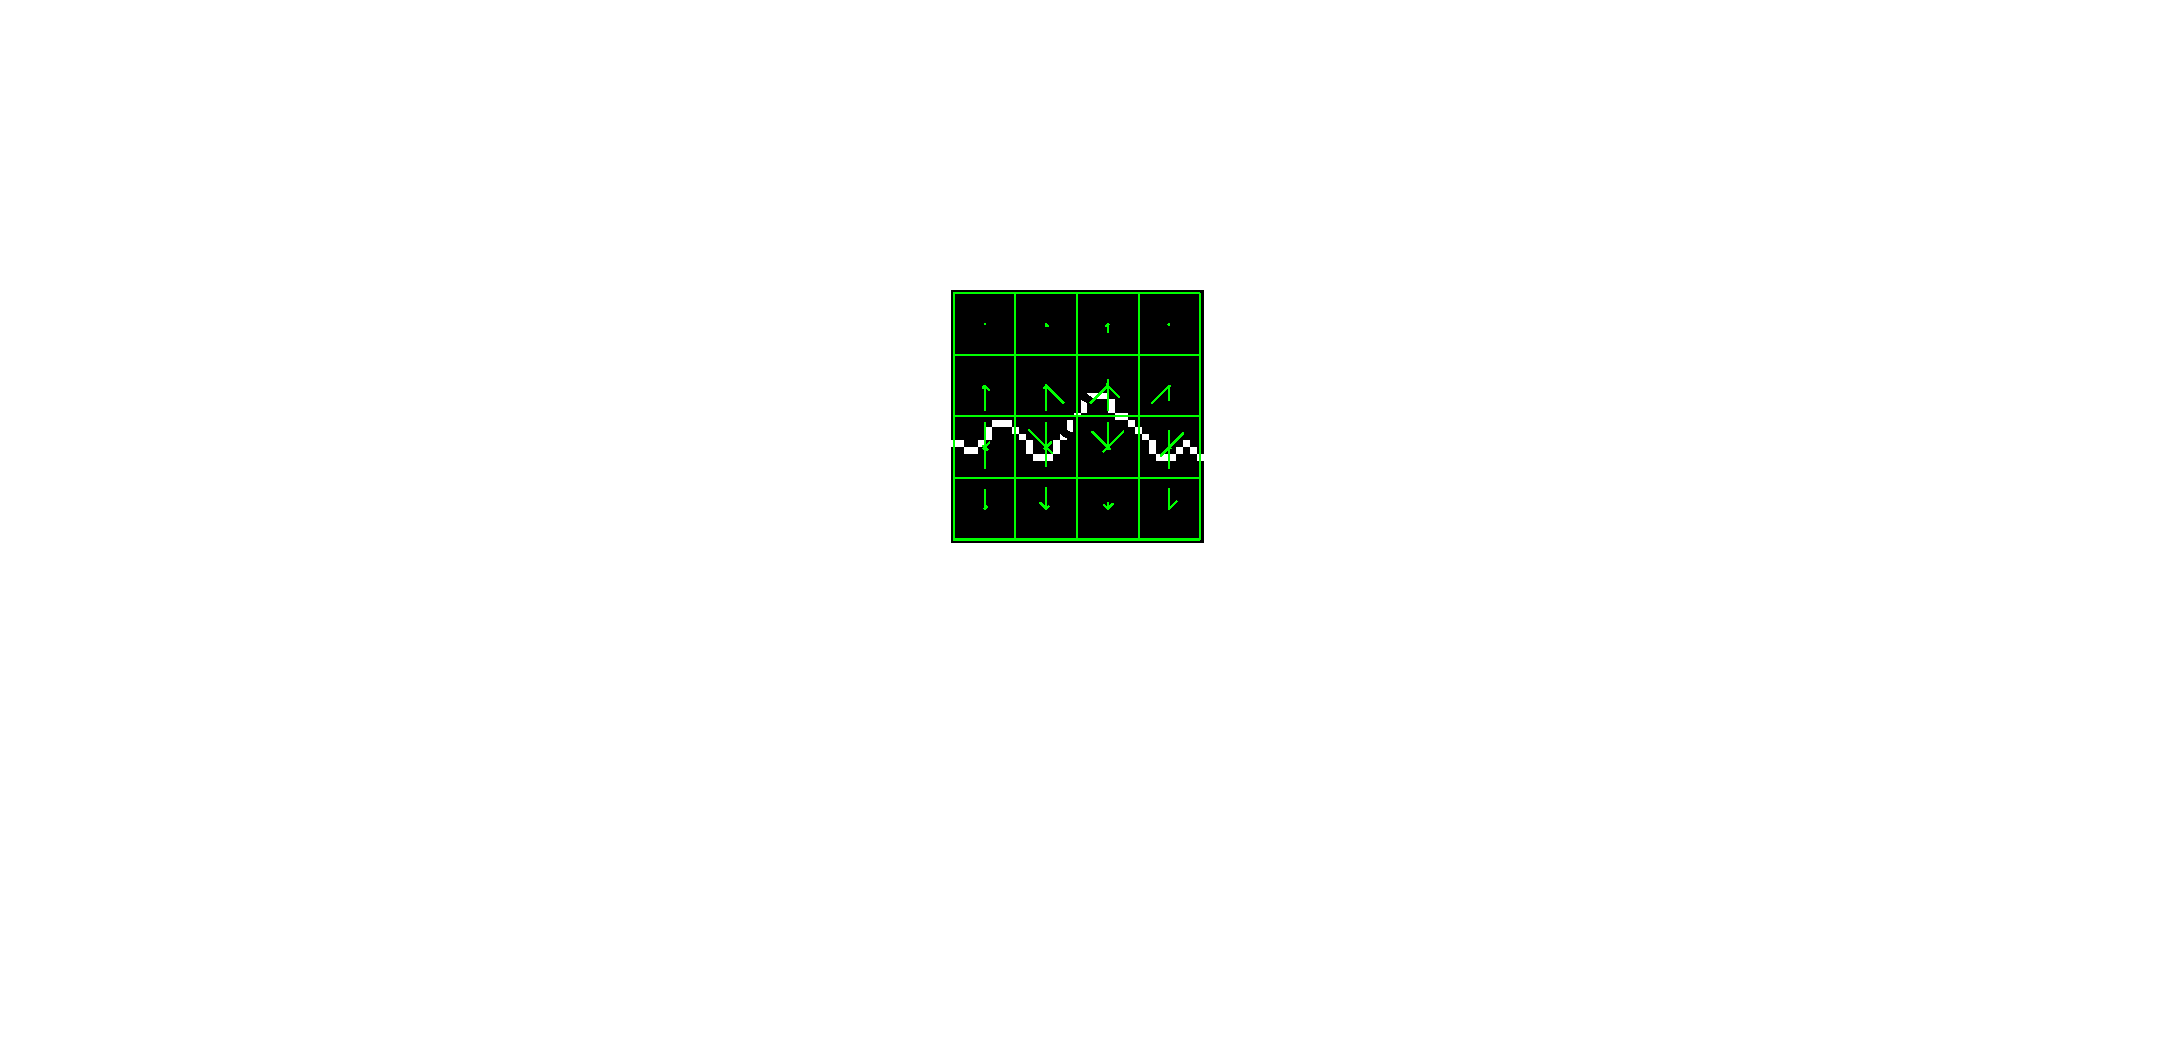
\includegraphics[width=16cm]{sampledescriptor.eps}
\caption{The local patch is located around a sample point plotted on the temporary signal. All the sample points are interpolated using the Bresenham algorithm. The 4x4 grid can be seen on the descriptor and also arrows showing the dominant gradient on each block.}
\label{fig:sampledescriptor}
\end{figure}


\subsubsection{Classification}

The classification is carried out by using the discriminative semi-supervised classification method, the Naive Bayes Nearest Neighbout (NBNN) \citep{Boiman2008}. % algorithm which can be described as follows.

\begin{equation}
\hat{C} = argmin_C \sum_{}^{} \left\lVert d_i - NN_C(d_i) \right\rVert ^2
\end{equation}

%BCI Simulation vs k-fold cross validation.  It is quite known and understood that because the same experience will not generate the same markers in the EEG, BCI Simulation is sometimes better suited to understand how the device will operate on a real online application (the graeat variability of BCI).

%%%%%%%%%%%%%%%%%%%%%%%%%%%%%%%%%%%%%%%%%%
\section{Results}

In Figure \ref{fig:subjectaveraged} the grand average (point-to-point) for all the subjects is shown.  The P300 characteristic curve can be seen particularly in subjects 2, and 6 and in a lesser extend in the remaining subjects. In order to obtain a valid binary classification on averaged signals, particular care was observed to avoid unbalanced samples, because that may introduce a bias in the classification procedure (signal variance is proportional to the square root of the number of samples and the procedure would be discriminating signals with different variances).Particularly in the case of the P300 response, the oddball paradigm requires that one of the stimulus need to be infrequent so that will unavoidably force that the data will be unbalanced (that is, an unequal number of trials in each condition).


\begin{figure}[H]
\centering
\includegraphics[width=16cm]{subjectaveraged.eps}
\caption{Point-To-Point grand averages of epochs obtained for hits (solid line) and no hits (dashed line) for each one of the 8 subjects for channel Cz. The P300 characteristic curve can be well identified on subjects 2 and 6.}
\label{fig:subjectaveraged}
\end{figure}

Results are shown in Table \ref{tab:results} where BCI accuracy
for the Cz channel is calculated and compared with the values obtained by the published of the dataset.  Additionally the best performing channel is informed and its accuracy value.  It is of particular interest that using this method, the best performing channel was not always Cz, and instead occipital channels PO8 and PO7 showed very good performance indeed \citep{Huggins2016,Jure2016}.

% (CITE TAYLOR AND  FRANCOS PAPER).

\begin{table}[H]
\caption{Results obtained for Accuracy levels by 3-fold cross validation. The values reported by the dataset publishers for Cz are reproduced here for comparison. Additionally, channel Cz BCI accuracies can be seen as well as the performance levels obtained for the BPC, the best performing channel for each subject.}
\centering
%% \tablesize{} %% You can specify the fontsize here, e.g.  \tablesize{\footnotesize}. If commented out \small will be used.
\begin{tabular}{ccccc}
\toprule
\textbf{Participants}	& \textbf{Original Cz}	& \textbf{ACC at Cz}	& \textbf{BPC}	& \textbf{Performance}\\
\midrule
1     &   0.84 &   0.79 & Cz  &   0.79 $\pm$ 0.01 \\
2     &   0.86 &   0.81 & PO7 &   0.93 $\pm$ 0.01 \\
3     &   0.87 &   0.78 & Cz  &   0.78 $\pm$ 0.03 \\
4     &   0.86 &   0.68 & PO8 &   0.90 $\pm$ 0.01 \\
5     &   0.86 &   0.80 & PO7 &   0.93 $\pm$ 0.01 \\
6     &   0.89 &   0.96 & Cz  &   0.96 $\pm$ 0.01 \\
7     &   0.89 &   0.78 & PO7 &   0.93 $\pm$ 0.01 \\
8     &   0.92 &   0.91 & PO7 &   1.00 $\pm$ 0.00 \\
\bottomrule
\end{tabular}
\label{tab:results}
\end{table}

The ITR, or BTR, in the case of reactive BCIs \citep{WolpawJonathanR2012} strongly depends on the amount of signal averaging required to transmit a valid and robust selection.  There is a trade-off that needs to be balanced between the required number of repetitions for each trial to guarantee robust transmission and the the achieved speed of transmission affected by the repetions.  As detailed in the table \ref{tab:singletrialreduction} this method is only reduced in a 20 percent in accuracy levels even by using only one sequence of repetitions.

\begin{table}[H]
\caption{Results obtained for Accuracy levels by performing a BCI simulation for the testing dataset. The BPC, best performing channel is shown and also performance levels for the 120, 60 and 12 repetitions. Finally the PR, performance reduction is described.  Almost all the subjects performed around 70\% even with by averaging 2 signals for each class.}
\centering
%% \tablesize{} %% You can specify the fontsize here, e.g.  \tablesize{\footnotesize}. If commented out \small will be used.
\begin{tabular}{cccccc}
\toprule
\textbf{Participants}	& \textbf{BPC}	& \textbf{ACC@120}	& \textbf{ACC@60}	&  \textbf{ACC@12} & \textbf{PR}\\
\midrule
1 & Cz &   0.80 &   0.82 &   0.72 & 9\% \\
2 & PO7 &   0.93 &   0.78 &   0.75 & 18\%\\
3 & Cz &   0.80 &   0.82 &   0.72 & 9\%\\
4 & PO8 &   0.93 &   0.78 &   0.65 & 29\%\\
5 & PO7 &   0.93 &   0.78 &   0.75 & 18\%\\
6 & Cz &   0.80 &   0.82 &   0.72 & 9\%\\
7 & PO7 &   0.93 &   0.78 &   0.75 & 18\%\\
8 & PO7 &   0.93 &   0.78 &   0.75 & 18\%\\
\bottomrule
\end{tabular}
\label{tab:singletrialreduction}
\end{table}

%%%%%%%%%%%%%%%%%%%%%%%%%%%%%%%%%%%%%%%%%%
%\section{Discussion}
%
%This method, different from other methods which is based on the nonlinearity of the gradient of histograms which can be used to detect 
%
%is also based on how the image look like.
%
%SNR of p300 and how to detect it
%
%Check if you can use this to detect any kind of transient signal.
%
%Compare if it is possible with the descriptors from one subject, discriminate the others.
%
%Channal identification based on the metric distance between the bags


%%%%%%%%%%%%%%%%%%%%%%%%%%%%%%%%%%%%%%%%%%
\section{Conclusion}

A method to characterize and classify EEG signals where the main characteristic can be both, rhythmic in nature as in motor imagery, and also transient in time space, like the P300 has been presented.

Although single trial classification was not perfectly achieved, it has been shown that this method could be applied with a P300 Speller Matrix application with increased ITR.

%Databases of descriptors.  Flexibility of the descriptor in terms of configuration and size (reference variants of SIFT on lower dimensiones).

The adaptive behaviour of the algorithm make is well suited when the shape of the pattern elicited by the P300 response, does not conform to the predicted structure.  This is because, the descriptors are directly based on how the signals actually looked like for the training and calibration step, and they do not require any prior knowledge about the signal.  This is of particular relevance for studies on outliers populations as may be the case for people who suffered some neuro-degenerative disease like Lou Gehrig's disease.

The expanding of the understanding of this tool in order to automatically classify patterns in EEG, that are specifically identified by their shapes, is a prospect future work to be considered.  It may also provide  assistance to physician or electroencephalographers to help them locate these EEG patterns particularly in long recording periods \citep{Hartman2005}, frequent in sleep research.

Moreover, this method can be used as an alternate \textit{BCI predictor} \citep{Clerc} or as a tool for artefact removal (which is performed on many occasions by visually inspecting the signal).

%%%%%%%%%%%%%%%%%%%%%%%%%%%%%%%%%%%%%%%%%%
%\subsection{Subsection}
%
%\subsubsection{Subsubsection}
%
%Bulleted lists look like this:
%\begin{itemize}[leftmargin=*,labelsep=4mm]
%\item	First bullet
%\item	Second bullet
%\item	Third bullet
%\end{itemize}
%
%Numbered lists can be added as follows:
%\begin{enumerate}[leftmargin=*,labelsep=3mm]
%\item	First item
%\item	Second item
%\item	Third item
%\end{enumerate}
%
%The text continues here.



%%%%%%%%%%%%%%%%%%%%%%%%%%%%%%%%%%%%%%%%%%
\vspace{6pt} 

%%%%%%%%%%%%%%%%%%%%%%%%%%%%%%%%%%%%%%%%%%
%% optional
%\supplementary{The following are available online at www.mdpi.com/link, Figure S1: title, Table S1: title, Video S1: title.}

%%%%%%%%%%%%%%%%%%%%%%%%%%%%%%%%%%%%%%%%%%
\acknowledgments{This project was supported by the ITBACyT-15 funding program issued by ITBA University.}

%%%%%%%%%%%%%%%%%%%%%%%%%%%%%%%%%%%%%%%%%%
\authorcontributions{This projects is part of a the first author's PhD Thesis which is directed by Juan Miguel Santos and codirected by Ana Julia Villar.}

%%%%%%%%%%%%%%%%%%%%%%%%%%%%%%%%%%%%%%%%%%
\conflictofinterests{The authors declare no conflict of interest.} 

%%%%%%%%%%%%%%%%%%%%%%%%%%%%%%%%%%%%%%%%%%
%% optional
\abbreviations{The following abbreviations are used in this manuscript:\\

\noindent EEG: electroencephalography\\
BCI: Brain Computer Interfaces\\
SNR: Signal to Noise Ratio\\
CNS: Central Nervous System\\
ALS: Amyotrophic Lateral Sclerosis\\
ERP: Event-Related Potential\\
P300: Positive deflection of an Event-Related Potential which occurs 300 ms after onset of stimuli\\
ITR: Information Transfer Rate}

%%%%%%%%%%%%%%%%%%%%%%%%%%%%%%%%%%%%%%%%%%
%% optional
%\appendixtitles{no} %Leave argument "no" if all appendix headings stay EMPTY (then no dot is printed after "Appendix A"). If the appendix sections contain a heading then change the argument to "yes".
%\appendixsections{multiple} %Leave argument "multiple" if there are multiple sections. Then a counter is printed ("Appendix A?). If there is only one appendix section then change the argument to ?one? and no counter is printed (?Appendix?).
%\appendix
%\section{}
%The appendix is an optional section that can contain details and data supplemental to the main text. For example, explanations of experimental details that would disrupt the flow of the main text, but nonetheless remain crucial to understanding and reproducing the research shown; figures of replicates for experiments of which representative data is shown in the main text can be added here if brief, or as Supplementary data. Mathemtaical proofs of results not central to the paper can be added as an appendix.
%
%\section{}
%All appendix sections must be cited in the main text. In the appendixes, Figures, Tables, etc. should be labeled starting with `A', e.g., Figure A1, Figure A2, etc. 

%%%%%%%%%%%%%%%%%%%%%%%%%%%%%%%%%%%%%%%%%%
% Citations and References in Supplementary files are permitted provided that they also appear in the reference list here. 
\bibliographystyle{mdpi}

%=====================================
% References, variant A: internal bibliography
%=====================================
%\renewcommand\bibname{References}
%\begin{thebibliography}{999}
% Reference 1
%\bibitem{ref-journal}
%Lastname, F.; Author, T. The title of the cited article. {\em Journal Abbreviation} {\bf 2008}, {\em 10}, 142-149.
% Reference 2
%\bibitem{ref-book}
%Lastname, F.F.; Author, T. The title of the cited contribution. In {\em The Book Title}; Editor, F., Meditor, A., Eds.; Publishing House: City, Country, 2007; pp. 32-58.
%\end{thebibliography}

%=====================================
% References, variant B: external bibliography
%=====================================
\bibliography{article}

%%%%%%%%%%%%%%%%%%%%%%%%%%%%%%%%%%%%%%%%%%
%% optional
%\sampleavailability{Samples of the compounds ...... are available from the authors.}

%%%%%%%%%%%%%%%%%%%%%%%%%%%%%%%%%%%%%%%%%%
\end{document}

